\clearpage
\subsection{SUSY\label{sec:interpretation}}

%Limits are set in the parameter space of a set of simplified models
%that characterise both third-generation squark production and
%compressed spectra scenarios, where the mass difference between the
%primary produced sparticle (e.g. a squark or a gluino) and the LSP is
%rather small. The \cls method~\cite{read,junk} is used to compute the
%limits, with the one-sided profile likelihood ratio as the test
%statistic~\cite{Cowan:2010js}.  The sampling distributions for the
%test statistic are built by generating pseudo-data from the likelihood
%function, using the respective maximum-likelihood values of the
%nuisance parameters under the background-only and
%signal-plus-background hypotheses.
% 
%Events samples for the simplified models are generated at leading
%order with \MADGRAPH~\cite{madgraph}. Inclusive, process-dependent,
%next-to-leading order calculations with next-to-leading logarithmic
%corrections~\cite{susy-nlo-nll} (NLO+NLL) of SUSY production cross
%sections are obtained with the program
%\PROSPINO~\cite{Beenakker:1996ch} and CTEQ6M~\cite{Pumplin:2002vw}
%parton distribution functions. The simulated signal events include
%multiple interactions per LHC bunch crossing (pileup) with the
%distribution of reconstructed vertices that match the one observed in
%data.
%
%The production and decay modes of the simplified models under
%consideration are summarised in Table~\ref{tab:sms}. 
%Also listed are the \njet and \nb bins that are considered for each
%interpretation.
%%The models \texttt{T1} and \texttt{T2} are used to characterise the
%%pair production of gluinos and first- or second-generation squarks,
%%respectively, depending on their mass as well as on the LSP mass. The
%%simplified models \texttt{T2tt}, \texttt{T2bb}, \texttt{T1tttt}, and
%%\texttt{T1bbbb} describe various production and decay mechanisms in
%%the context of third-generation squarks. 
%
%%Appendix~\ref{app:gains} shows the expected limits in the model
%%\texttt{T1} when considering an inclusive jet multiplicity bin, $\njet
%%\geq 2$, just the exclusive jet multiplicity bin, \njethigh, and the
%%combination of the two exclusive jet multiplicity bins, \njetlow and
%%\njethigh, in the Figs.~\ref{fig:gains-incl}, \ref{fig:gains-high},
%%and \ref{fig:gains-both}. Significant gains of are made when
%%considering the higher or both exclusive \njet bins, especially in the
%%reach to higher LSP masses.
%
%Experimental uncertainties on the SM background predictions, the
%integrated luminosity measurement, and the total acceptance times
%efficiency of the selection for the considered signal model are
%included in the calculation of the limit.
%
%%Experimental uncertainties on the SM background predictions
%%($10-30\%$), the luminosity measurement (4.4\%), and the total
%%acceptance times efficiency of the selection for the considered signal
%%model (12\%$-$18\%) are included in the calculation of the limit.
%%Signal efficiency in the kinematic region defined by $0 <
%%m_{\sGlu(\sQua)} - m_{\textrm{LSP}} < 175\gev$ or $m_{\sGlu(\sQua)} <
%%300\gev$ is strongly affected by the presence of initial-state
%%radiation. We do not consider this region in which direct (\ie,
%%non-ISR induced) production is kinematically forbidden due to the
%%$\scalht > 275\GeV$ requirement. Given the large associated
%%uncertainties, no interpretation is provided for this kinematic
%%region. In the case of model \texttt{T1tttt}, for which pair-produced
%%gluinos decay to \ttbar pairs and the LSP, the region $0 < m_{\sGlu} -
%%m_{\textrm{LSP}} < 400\gev$ is not considered.
%
%\begin{table}[h!]
%  \caption{The first two columns specify the model and its
%    production and decay. The next column specifies the event
%    categories (in terms of \njet and
%    \nb) considered for each interpretation. The last 
%    two columns indicate the search sensitivity for each model,
%    where $m_{\sq(\sGlu)}^{\textrm{best}}$ and
%    $m_{\textrm{LSP}}^{\textrm{best}}$ represent the largest mass 
%    beyond which no limit can be set for squarks/gluinos and the LSP,
%    respectively. The exclusion range for $m_{\sq(\sGlu)}$ is bounded
%    from below by the kinematic region considered for each model, as
%    defined in the text. The quoted estimates are determined 
%    conservatively from the observed exclusion based on the
%    theoretical production cross section minus $1\sigma$
%    uncertainty. 
%    %For model \texttt{T2tt}, the search is at the threshold of
%    %sensitivity for the considered ($m_{\sQua},m_{\rm LSP}$) parameter
%    %space, as discussed in the text. 
%  }  
%  \label{tab:sms}
%  \centering
%  \footnotesize
%  \begin{tabular}{ llcccc }
%    \hline
%    Model
%    & Production/decay
%    & Event categories
%    & Limit plot
%    & $m_{\sq(\sGlu)}^{\textrm{best}}$~(GeV) 
%    & $m_{\textrm{LSP}}^{\textrm{best}}$~(GeV) 
%    \\ [0.5ex]
%    \hline
%    \texttt{T2cc}
%    &
%    $\textrm{pp}\,\rightarrow\,\sTop\sTop\,\rightarrow\,\textrm{c}\chiz\bar{\textrm{c}}\chiz$
%    & ($\le3$,0), ($\ge4$,0), ($\ge4$,1)
%    & \ref{fig:limits-t2cc-obs}
%    & -
%    & n/a
%    \\
%%    \texttt{T1}
%%    &
%%    $\textrm{pp}\,\rightarrow\,\sGlu\sGlu\,\rightarrow\,\textrm{q}\bar{\textrm{q}}\chiz\textrm{q}\bar{\textrm{q}}\chiz$
%%    & $\geq4$
%%    & 0
%%    & \ref{fig:t1}
%%    & 950
%%    & 450
%%    \\
%%    \texttt{T2}
%%    & 
%%    $\textrm{pp}\,\rightarrow\,\sQua\sQua\,\rightarrow\,\textrm{q}\chiz\bar{\textrm{q}}\chiz$
%%    & 2--3
%%    & 0
%%    & \ref{fig:t2}
%%    & 775
%%    & 325
%%    \\
%%    \texttt{T2tt} 
%%    & 
%%    $\textrm{pp}\,\rightarrow\,\sTop\sTop\,\rightarrow\,\textrm{t}\chiz\bar{\textrm{t}}\chiz$
%%    & $\geq4$
%%    & 1,2
%%    & \ref{fig:t2tt-1d}
%%    & $-$ 
%%    & $-$
%%    \\ 
%%    \texttt{T2bb}
%%    & 
%%    $\textrm{pp}\,\rightarrow\,\sBot\sBot\,\rightarrow\,\textrm{b}\chiz\bar{\textrm{b}}\chiz$
%%    & 2--3
%%    & 1,2
%%    & \ref{fig:t2bb}
%%    & 600
%%    & 200
%%    \\
%%    \texttt{T1tttt} 
%%    &
%%    $\textrm{pp}\,\rightarrow\,\sGlu\sGlu\,\rightarrow\,\textrm{t}\bar{\textrm{t}}\chiz\textrm{t}\bar{\textrm{t}}\chiz$ 
%%    & $\geq4$
%%    & 2,3,$\geq4$
%%    & \ref{fig:t1tttt}
%%    & 950
%%    & 325
%%    \\
%%    \texttt{T1bbbb} 
%%    & 
%%    $\textrm{pp}\,\rightarrow\,\sGlu\sGlu\,\rightarrow\,\textrm{b}\bar{\textrm{b}}\chiz\textrm{b}\bar{\textrm{b}}\chiz$
%%    & $\geq4$
%%    & 2,3,$\geq4$
%%    & \ref{fig:t1bbbb}
%%    & 1125
%%    & 650
%%    \\
%    \hline
%  \end{tabular}
%\end{table}
%
%\fixme{TEXT REFLECTS USUAL PRESENTATION OF LIMIT PLOTS - ALL RELEVANT
%  INFORMATION IN SHOWN IN REFERENCED FIGURES FOR T2CC - TO BE UPDATED.}
%Figures~\ref{fig:limits-t2cc-exp} and \ref{fig:limits-t2cc-obs} show
%the upper limit on the cross section at 95\% CL as a function of
%$m_{\sq}$ or $m_{\gl}$ and $m_{\rm LSP}$ for various simplified
%models. The point-to-point fluctuations are due to the finite number
%of pseudo-experiments used to determine the observed upper limit. The
%solid thick black line indicates the observed exclusion region
%assuming NLO+NLL~\cite{Beenakker:1996ch, susy-nlo-nll} SUSY cross
%section for squark pair production in the limit of very massive
%gluinos (or vice versa). The thin black lines represent the observed
%excluded region when varying the cross section by its theoretical
%uncertainty. The dashed purple lines indicate the median (thick line)
%$\pm 1 \sigma$ (thin lines) expected exclusion regions.
%
%%Figure~\ref{fig:t2cc-1d} shows the observed upper limit at 95\% CL on
%%the production cross section as a function of the top squark mass
%%($m_{\sTop}$) for the model \texttt{T2cc} when considering two
%%different \sTop-\chiz mass splittings of $\Delta m = 10\gev$ (left)
%%and $\Delta m = 80\gev$ (right). The observed upper limit (95\% CL) on
%%the production cross section is shown as a function of $m_{\sTop}$
%%(solid line), along with the expected upper limit and
%%$\mathbf{\pm2}\sigma$ {\bf experimental uncertainties} (long-dashed
%%line with shaded band), and the NLO+NLL top squark pair-production
%%cross section and theoretical uncertainties (dotted line with shaded
%%band).
%
%Figure~\ref{fig:t2cc-best-fit} shows the \scalht-binned observed data
%yields and expectations for the hadronic sample, as determined by a
%simultaneous fit to all data samples under the signal+background
%hypothesis. The observed event yields in data (black dots), the SM
%expectations (dark blue) and the sum of the SM backgrounds and signal
%expectation (pink) are shown. The signal expectations are for the best
%fit model \texttt{T2cc} with $m_{\sq} = 250\GeV$ and $m_{\text{LSP}} =
%230\GeV$. Three event categories are considered by the fit: (Top)
%\njetlow and $\nb = 0$, (Middle) \njethigh and $\nb = 0$, (Bottom)
%\njethigh and $\nb = 1$. The fit is performed (Left) for each
%individual event category or (Right) simultaneously across all three
%event categories.
%
%\begin{figure}[h!]
%  \begin{center}
%    \subfigure[$+1\sigma$ experimental, relative]{
%      \includegraphics[width=0.45\textwidth,page=3,trim=40 50 20 70,clip=true]{figures/limits/v0/exp/CLs_frequentist_T2cc_2012dev_0b_le3j_0b_ge4j_1b_ge4j_xsLimit_relative}
%    } \quad
%    \subfigure[$+1\sigma$ experimental, excluded points]{
%      \includegraphics[width=0.45\textwidth,page=3,trim=40 50 20 70,clip=true]{figures/limits/v0/exp/CLs_frequentist_T2cc_2012dev_0b_le3j_0b_ge4j_1b_ge4j_xsLimit_simpleExcl}
%    } \\
%    \subfigure[Nominal, relative]{
%      \includegraphics[width=0.45\textwidth,page=1,trim=40 50 20 70,clip=true]{figures/limits/v0/exp/CLs_frequentist_T2cc_2012dev_0b_le3j_0b_ge4j_1b_ge4j_xsLimit_relative}
%    } \quad 
%    \subfigure[Nominal, excluded points]{
%      \includegraphics[width=0.45\textwidth,page=1,trim=40 50 20 70,clip=true]{figures/limits/v0/exp/CLs_frequentist_T2cc_2012dev_0b_le3j_0b_ge4j_1b_ge4j_xsLimit_simpleExcl}
%    } \\
%    \subfigure[$-1\sigma$ experimental, relative]{
%      \includegraphics[width=0.45\textwidth,page=2,trim=40 50 20 70,clip=true]{figures/limits/v0/exp/CLs_frequentist_T2cc_2012dev_0b_le3j_0b_ge4j_1b_ge4j_xsLimit_relative}
%    } \quad 
%    \subfigure[$-1\sigma$ experimental, excluded points]{
%      \includegraphics[width=0.45\textwidth,page=2,trim=40 50 20 70,clip=true]{figures/limits/v0/exp/CLs_frequentist_T2cc_2012dev_0b_le3j_0b_ge4j_1b_ge4j_xsLimit_simpleExcl}
%    } \\
%    \caption{\label{fig:limits-t2cc-exp} \fixme{TEMPORARY PLACE
%        HOLDERS FOR THE FINAL LIMIT PLOT. HOWEVER, ALL RELEVANT
%        INFORMATION IS CONTAINED HERE.} Expected limits for the model 
%      \texttt{T2cc}. In the left column, the plots show the upper
%      limit on the production cross section relative to the
%      theoretical value. In the right column, the plots show the mass
%      points that are excluded (marked red). In all plots, the yellow
%      line should be ignored. The expected limits are shown in the
%      middle row, with limits corresponding to the $+1\sigma$ and
%      $+1\sigma$ variations in the experimental uncertainties shown
%      top and bottom, respectively. }
%  \end{center}
%\end{figure}
%
\begin{figure}[h!]
  \begin{center}
    \subfigure[Expected, relative]{
      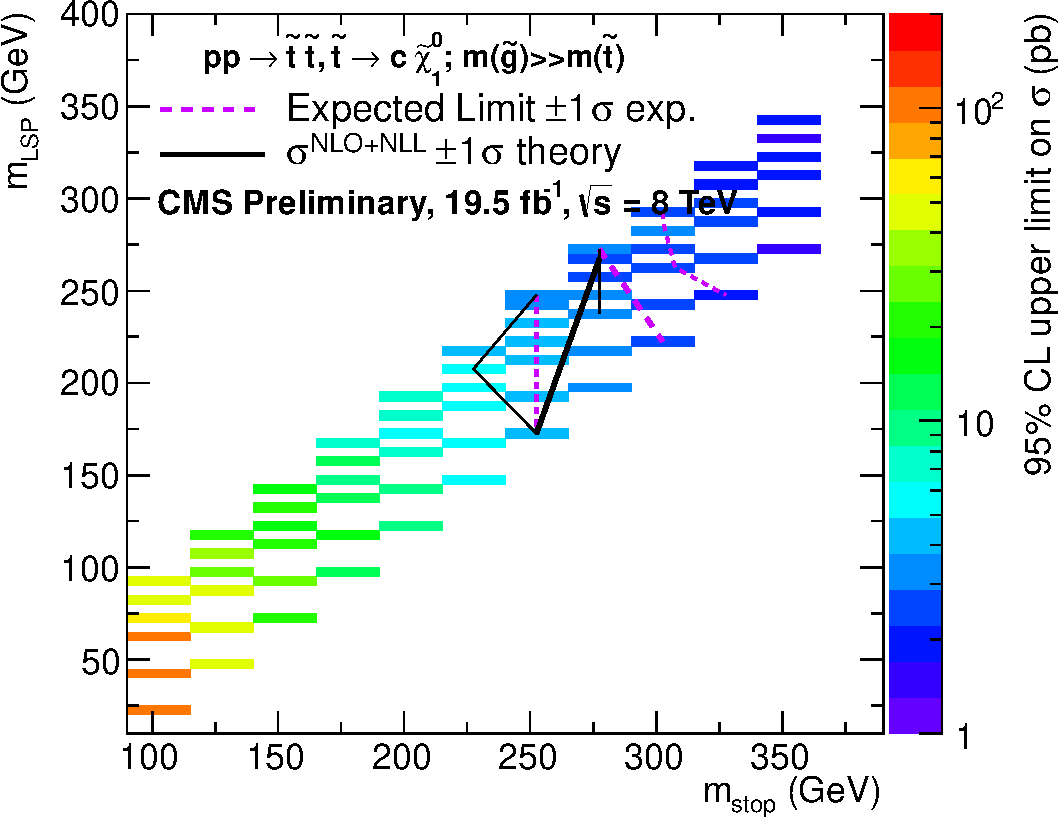
\includegraphics[width=0.45\textwidth,clip=true]{figures/limits/merged/T2cc/v2/CLs_frequentist_T2cc_2012pf_0b_le3j_0b_ge4j_1b_ge4j_xsLimit}
    } \quad 
    \subfigure[Expected, excluded points]{
      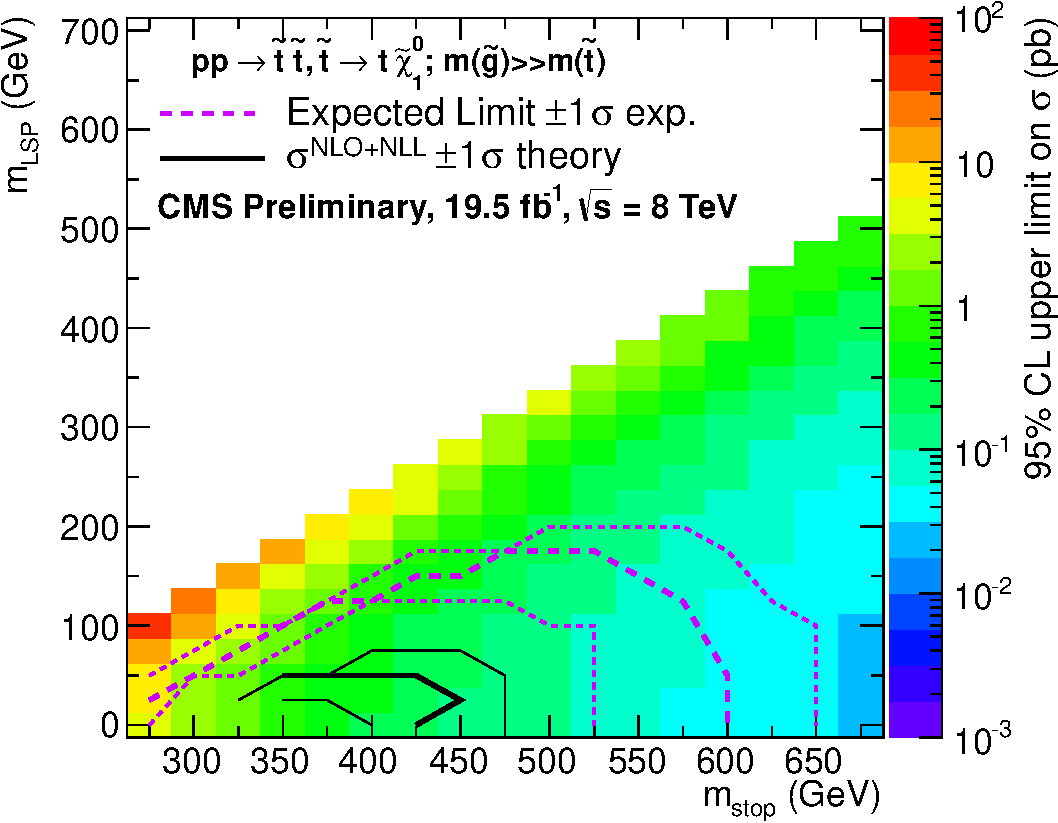
\includegraphics[width=0.45\textwidth,clip=true]{figures/limits/merged/T2tt/v6/CLs_frequentist_T2tt_2012pf_1b_ge4j_2b_ge4j_xsLimit.pdf}
    } \\
%    \subfigure[Observed, relative]{
%      \includegraphics[width=0.45\textwidth,page=4,trim=40 50 20 70,clip=true]{figures/limits/v0/obs/CLs_frequentist_T2cc_2012dev_0b_le3j_0b_ge4j_1b_ge4j_xsLimit_relative}
%    } \quad 
%    \subfigure[Observed, excluded points]{
%      \includegraphics[width=0.45\textwidth,page=4,trim=40 50 20 70,clip=true]{figures/limits/v0/obs/CLs_frequentist_T2cc_2012dev_0b_le3j_0b_ge4j_1b_ge4j_xsLimit_simpleExcl}
%    } \\
    \caption{\label{fig:limits-t2cc-obs} Expected and observed limits
      for the model \texttt{T2cc}. In the left column, the plots show
      the upper limit on the production cross section relative to the 
      theoretical value. In the right column, the plots show the mass
      points that are excluded (marked red). In all plots, the yellow
      line should be ignored. The expected limits are shown in the
      top row, the observed limits in the bottom row. }
  \end{center}
\end{figure}

\begin{figure*}[t!]
  \begin{center}
    \subfigure[\njethigh, $\nb = 1$, simultaneous fit]{
      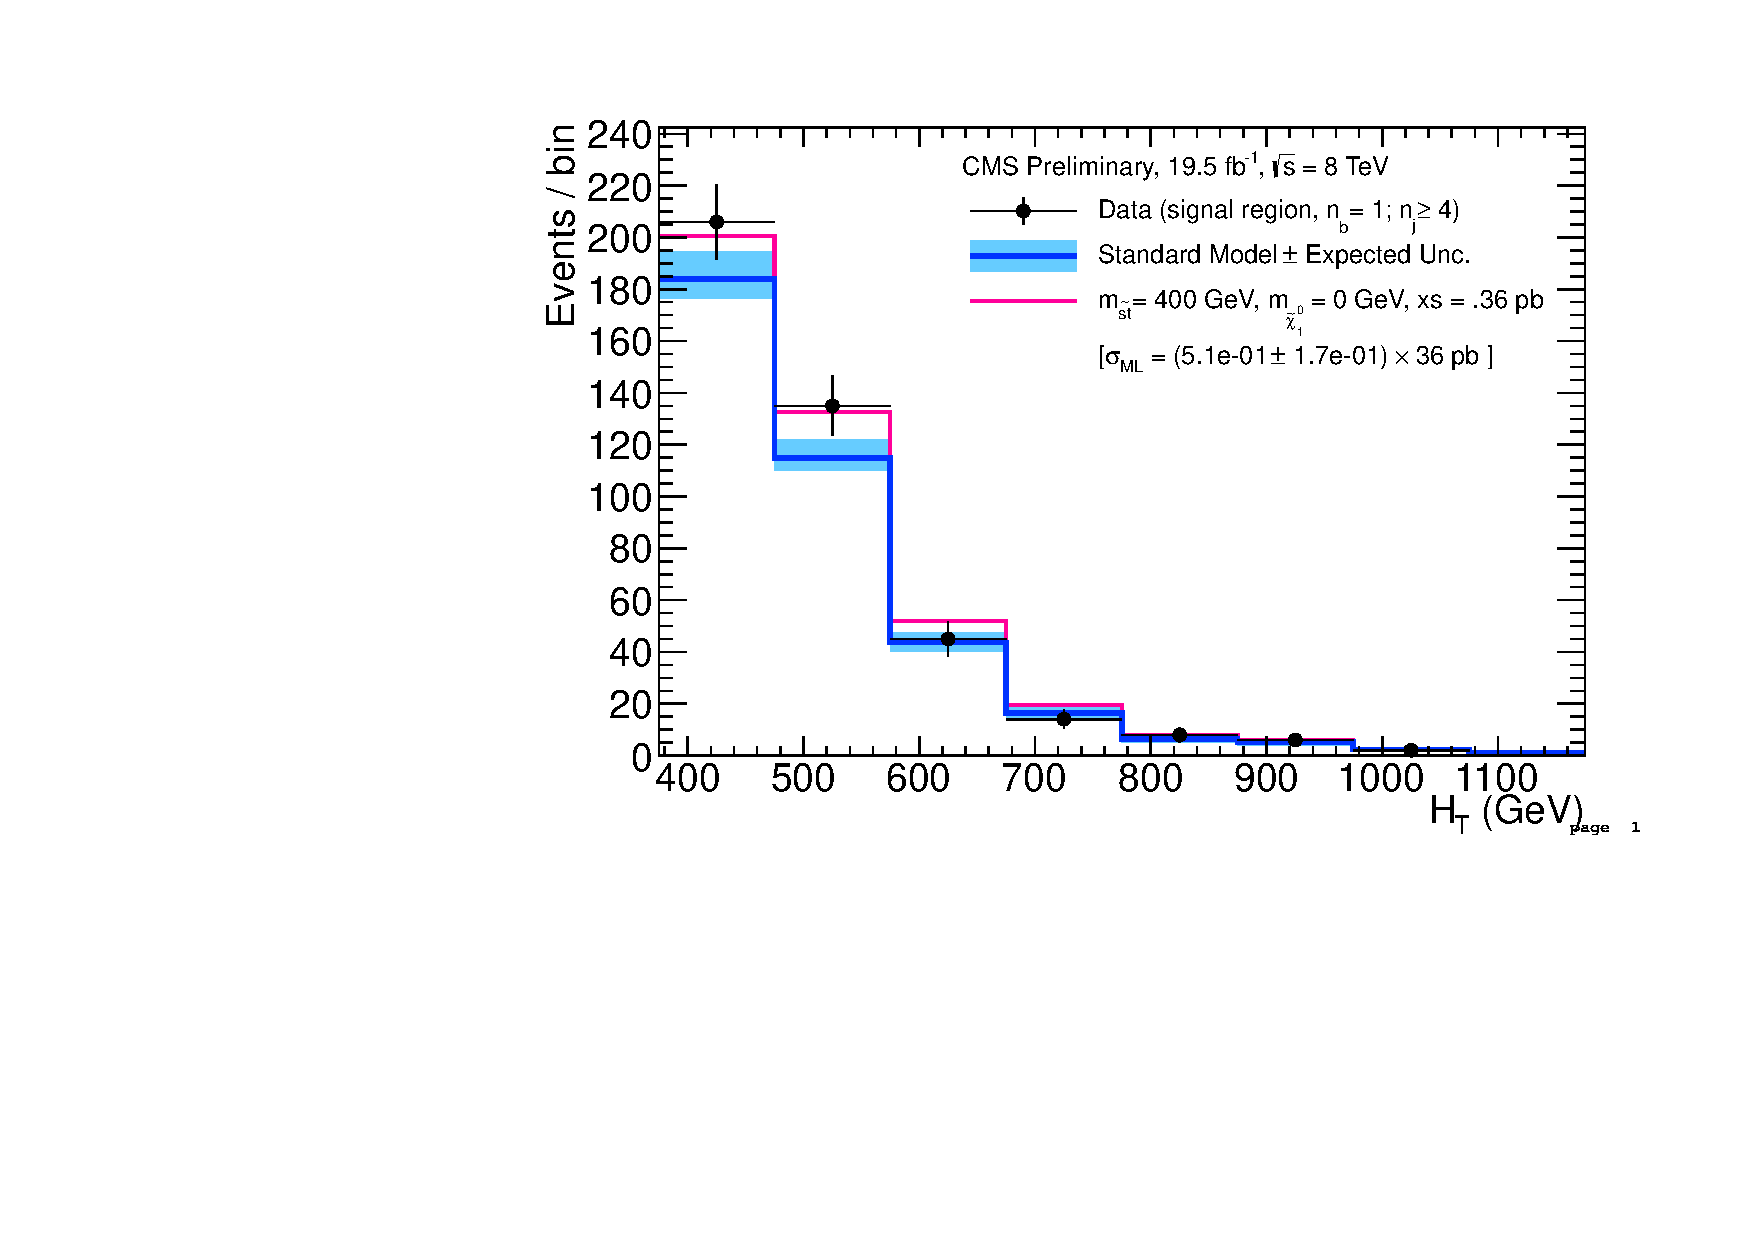
\includegraphics[width=0.45\textwidth]{figures/fit/v22/wSignal/400_0/bestFit_2012pf_RQcdZero_fZinvAll_1b_ge4j-1hp_2b_ge4j-1h_signal_sel1b_ge4j}
    } 
    \subfigure[\njethigh, $\nb = 2$, simultaneous fit]{
      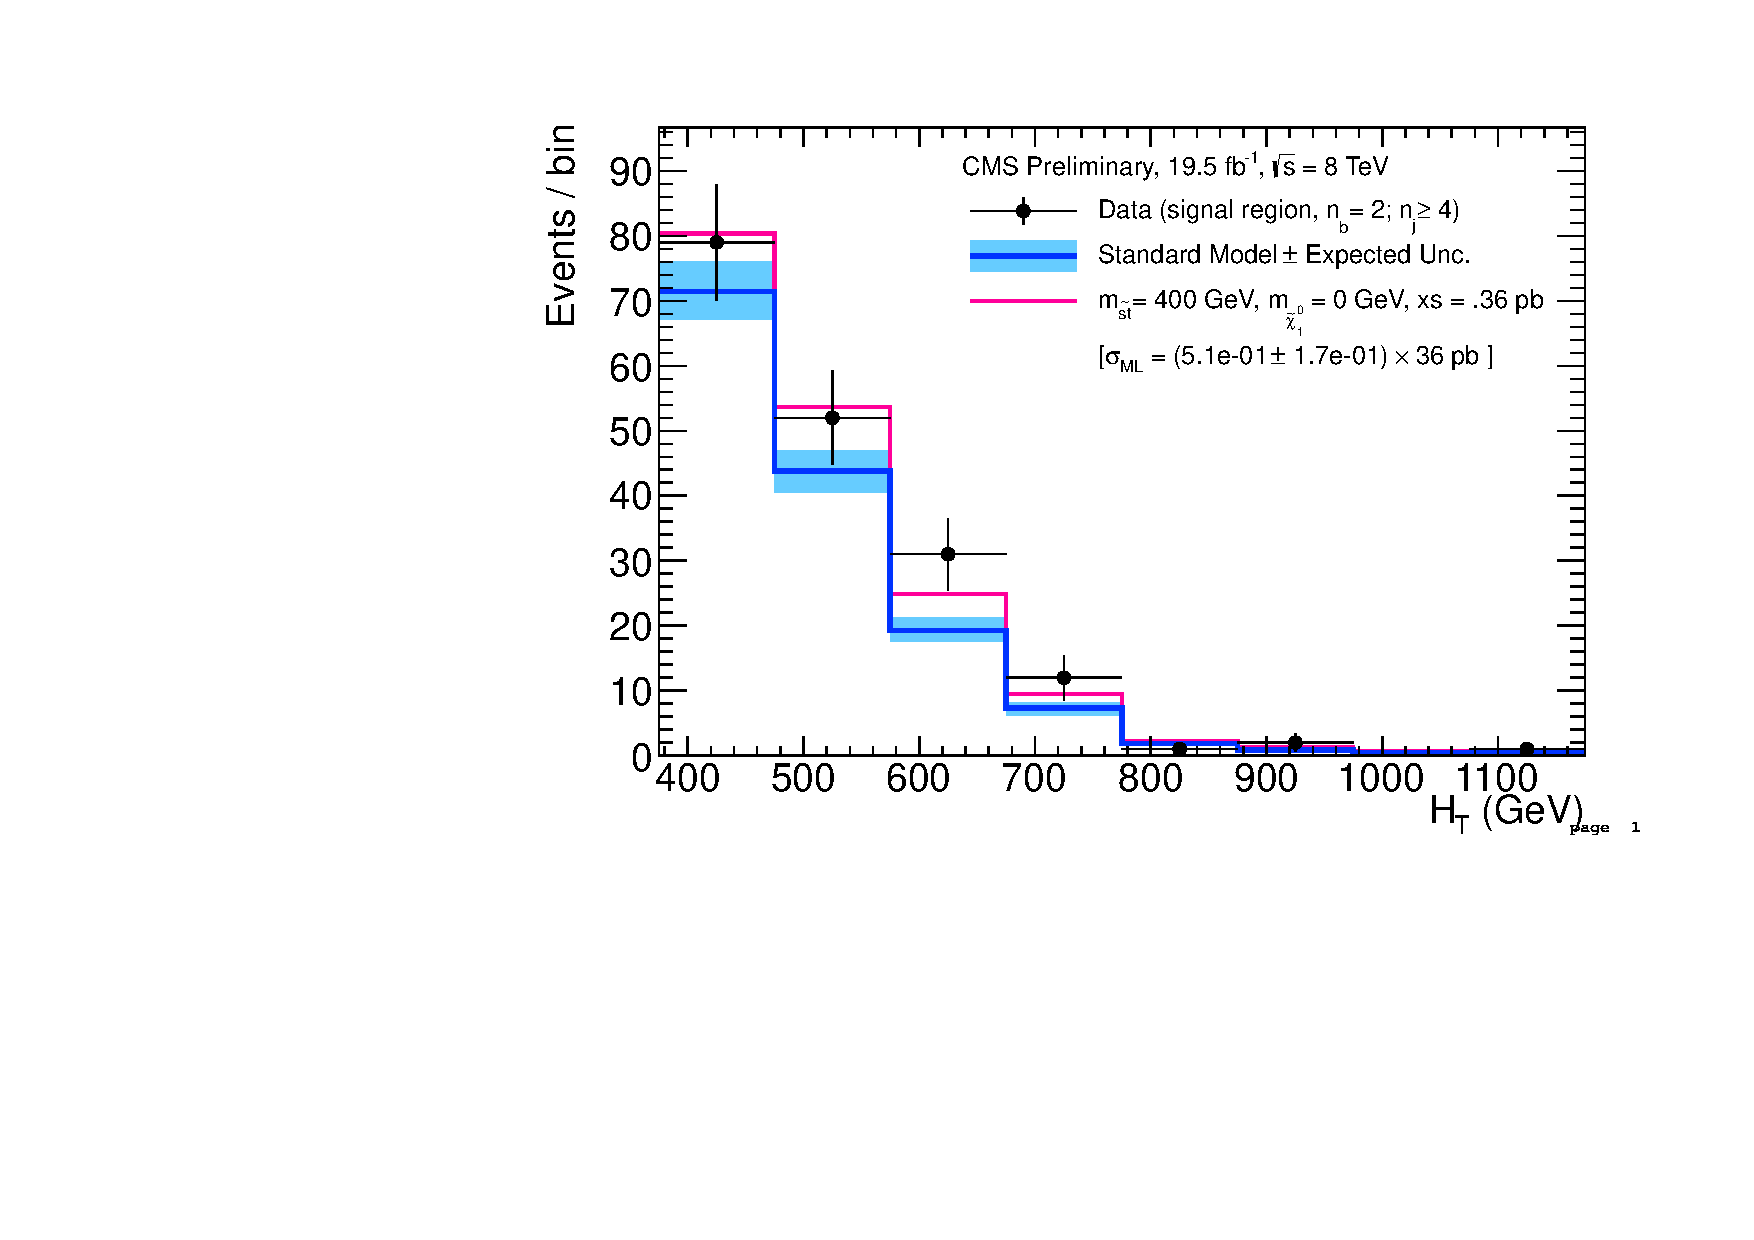
\includegraphics[width=0.45\textwidth]{figures/fit/v22/wSignal/400_0/bestFit_2012pf_RQcdZero_fZinvAll_1b_ge4j-1hp_2b_ge4j-1h_signal_sel2b_ge4j}
    } \\
    \subfigure[\njethigh, $\nb = 1$, simultaneous fit]{
      \includegraphics[width=0.45\textwidth,page=13]{figures/fit/v22/stackedSig/400_0/bestFit_2012pf_RQcdZero_fZinvAll_1b_ge4j-1p_2b_ge4j-1_sel1b_ge4j_smOnly.pdf}
    } 
    \subfigure[\njethigh, $\nb = 2$, simultaneous fit]{
      \includegraphics[width=0.45\textwidth,page=9]{figures/fit/v22/stackedSig/400_0/bestFit_2012pf_RQcdZero_fZinvAll_1b_ge4j-1p_2b_ge4j-1_sel2b_ge4j_smOnly.pdf}
    } \\
    \subfigure[Upper Limit on signal stength, simultaneous fit]{
      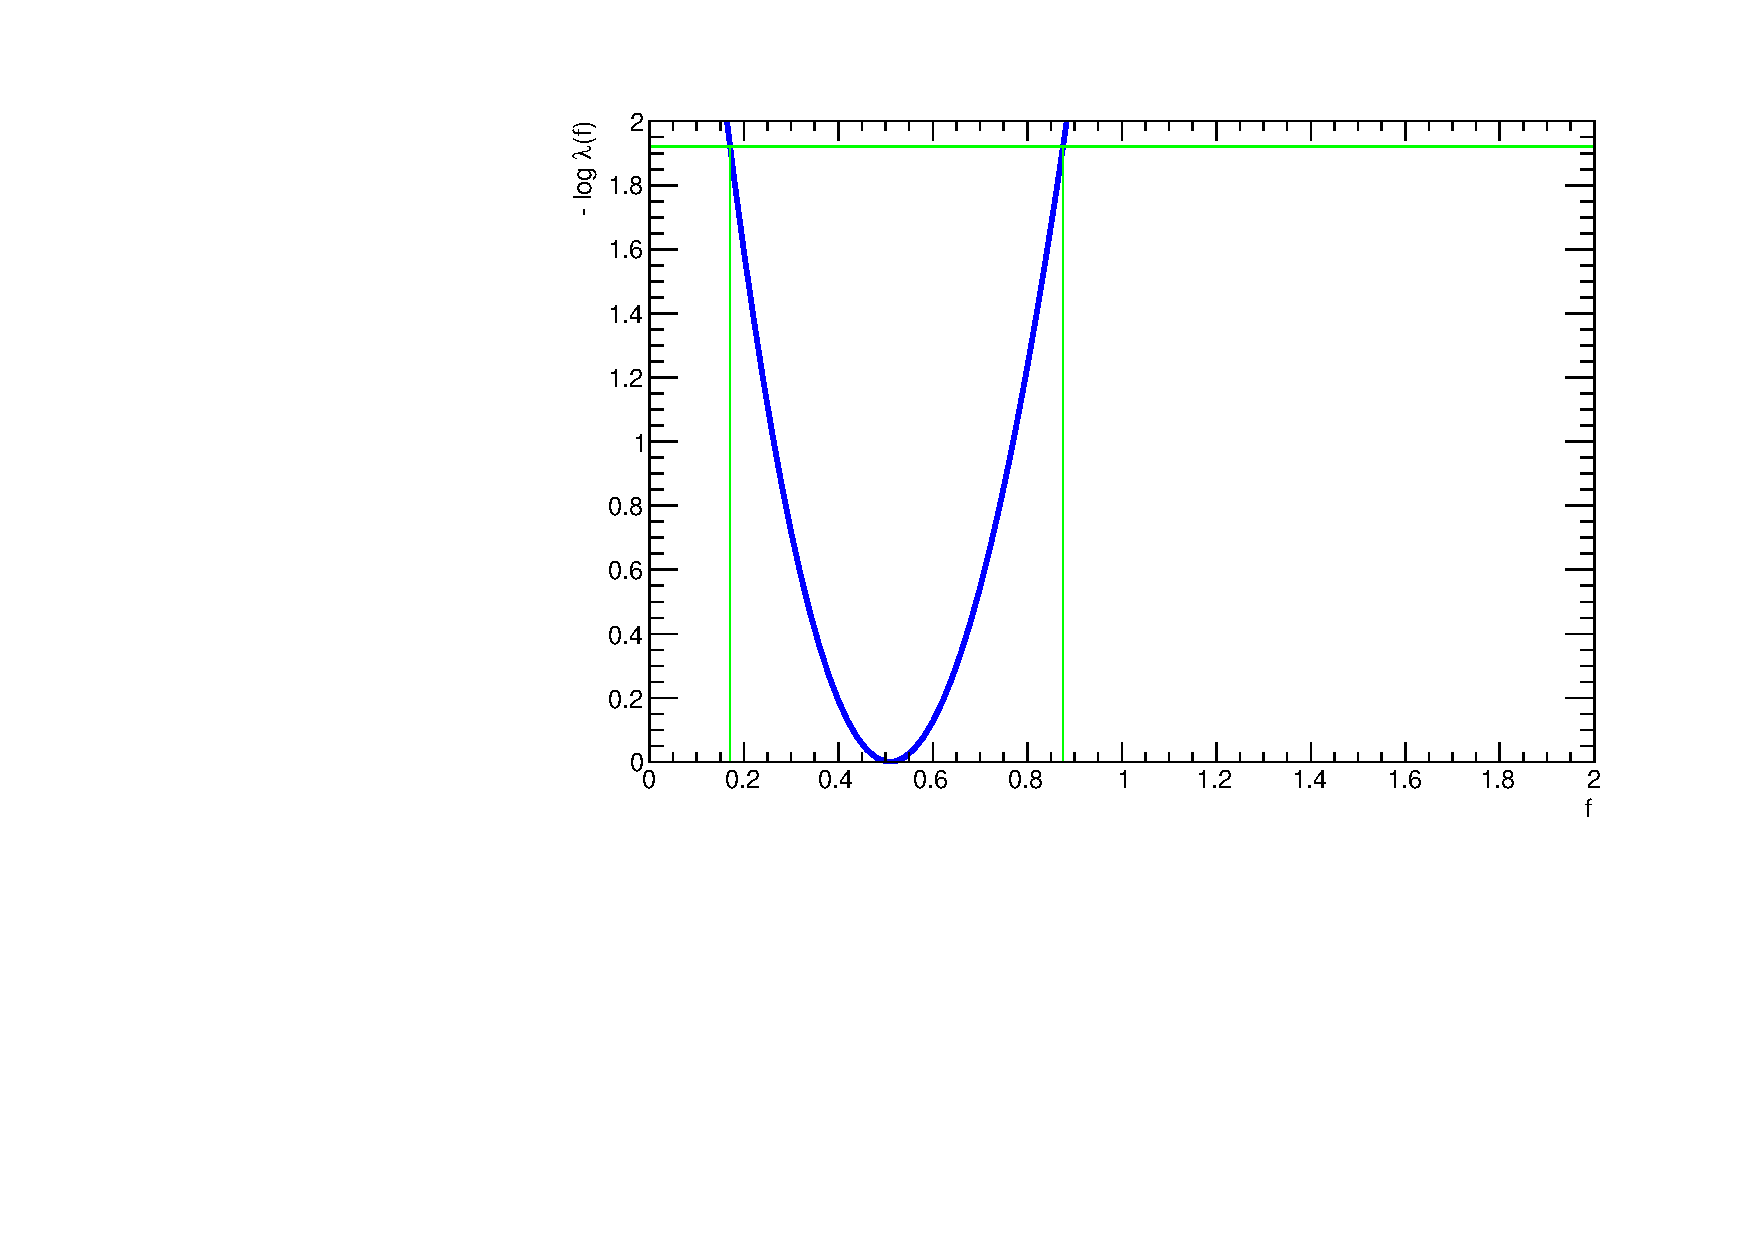
\includegraphics[width=0.45\textwidth]{figures/fit/v22/wSignal/400_0/intervalPlot_2012pf_RQcdZero_fZinvAll_1b_ge4j-1hp_2b_ge4j-1h_signal_95}
    } \\
    \caption{\label{fig:t2cc-best-fit} Comparison of
      the \scalht-binned observed data yields and expectations for the
      hadronic sample, as determined by a simultaneous fit to all data
      samples under the signal plus SM background hypothesis. The
      observed event yields in data (black dots), the SM expectations
      (dark blue solid line), and the signal expectations (pink solid
      line), as determined by the simultaneous fit, are shown. The
      signal model is \texttt{T2cc} with $m_{\sq} = 250\GeV$ and
      $m_{\text{LSP}} = 230\GeV$. Three event categories are
      considered: (Top) \njethigh and $\nb = 0$, (Middle) \njethigh and
      $\nb = 0$, (Bottom) \njethigh and $\nb = 1$. The fit is
      performed (Left) for each individual event category or (Right)
      simultaneously across all three event categories.}
  \end{center}
\end{figure*}

\begin{figure*}[t!]
  \begin{center}
    \subfigure[\njethigh, $\nb = 1$, simultaneous fit]{
      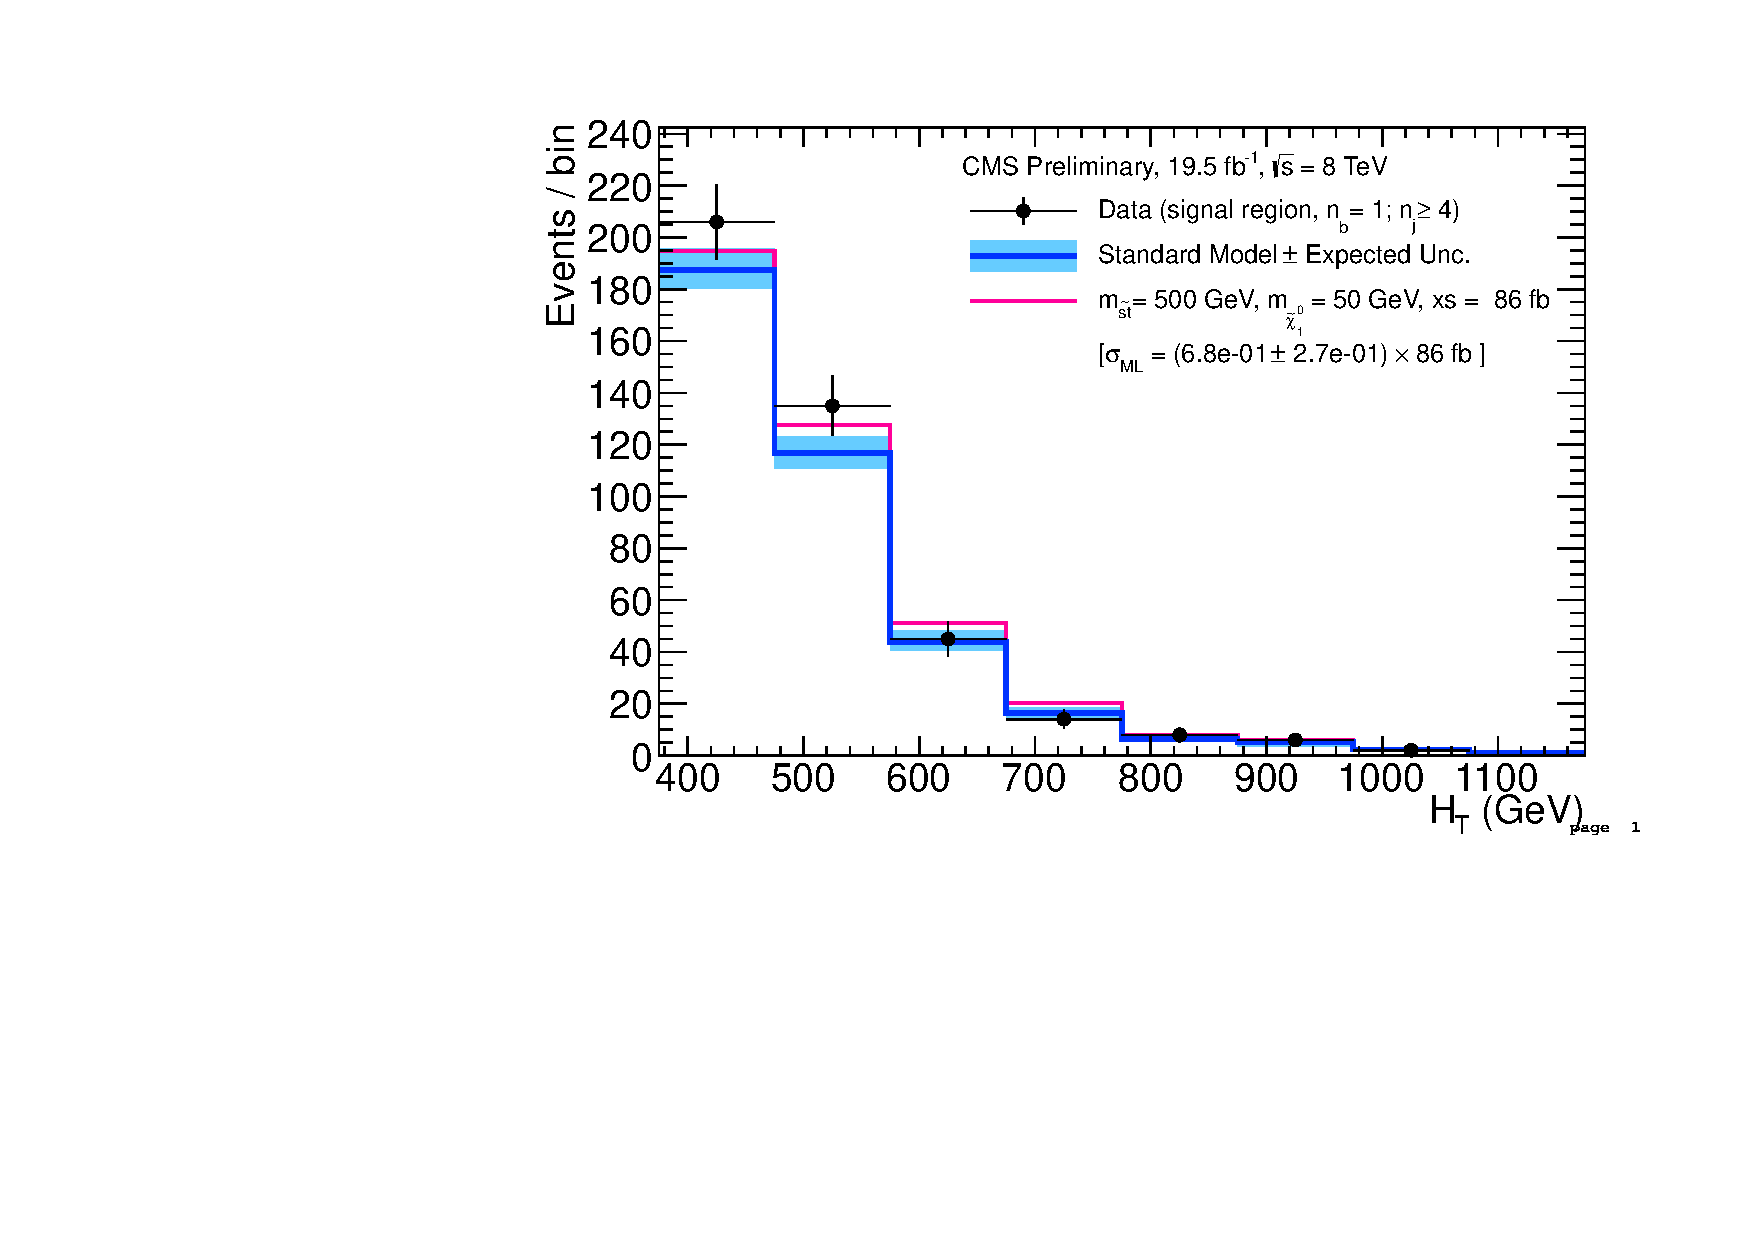
\includegraphics[width=0.45\textwidth]{figures/fit/v22/wSignal/500_50/bestFit_2012pf_RQcdZero_fZinvAll_1b_ge4j-1hp_2b_ge4j-1h_signal_sel1b_ge4j}
    } 
    \subfigure[\njethigh, $\nb = 2$, simultaneous fit]{
      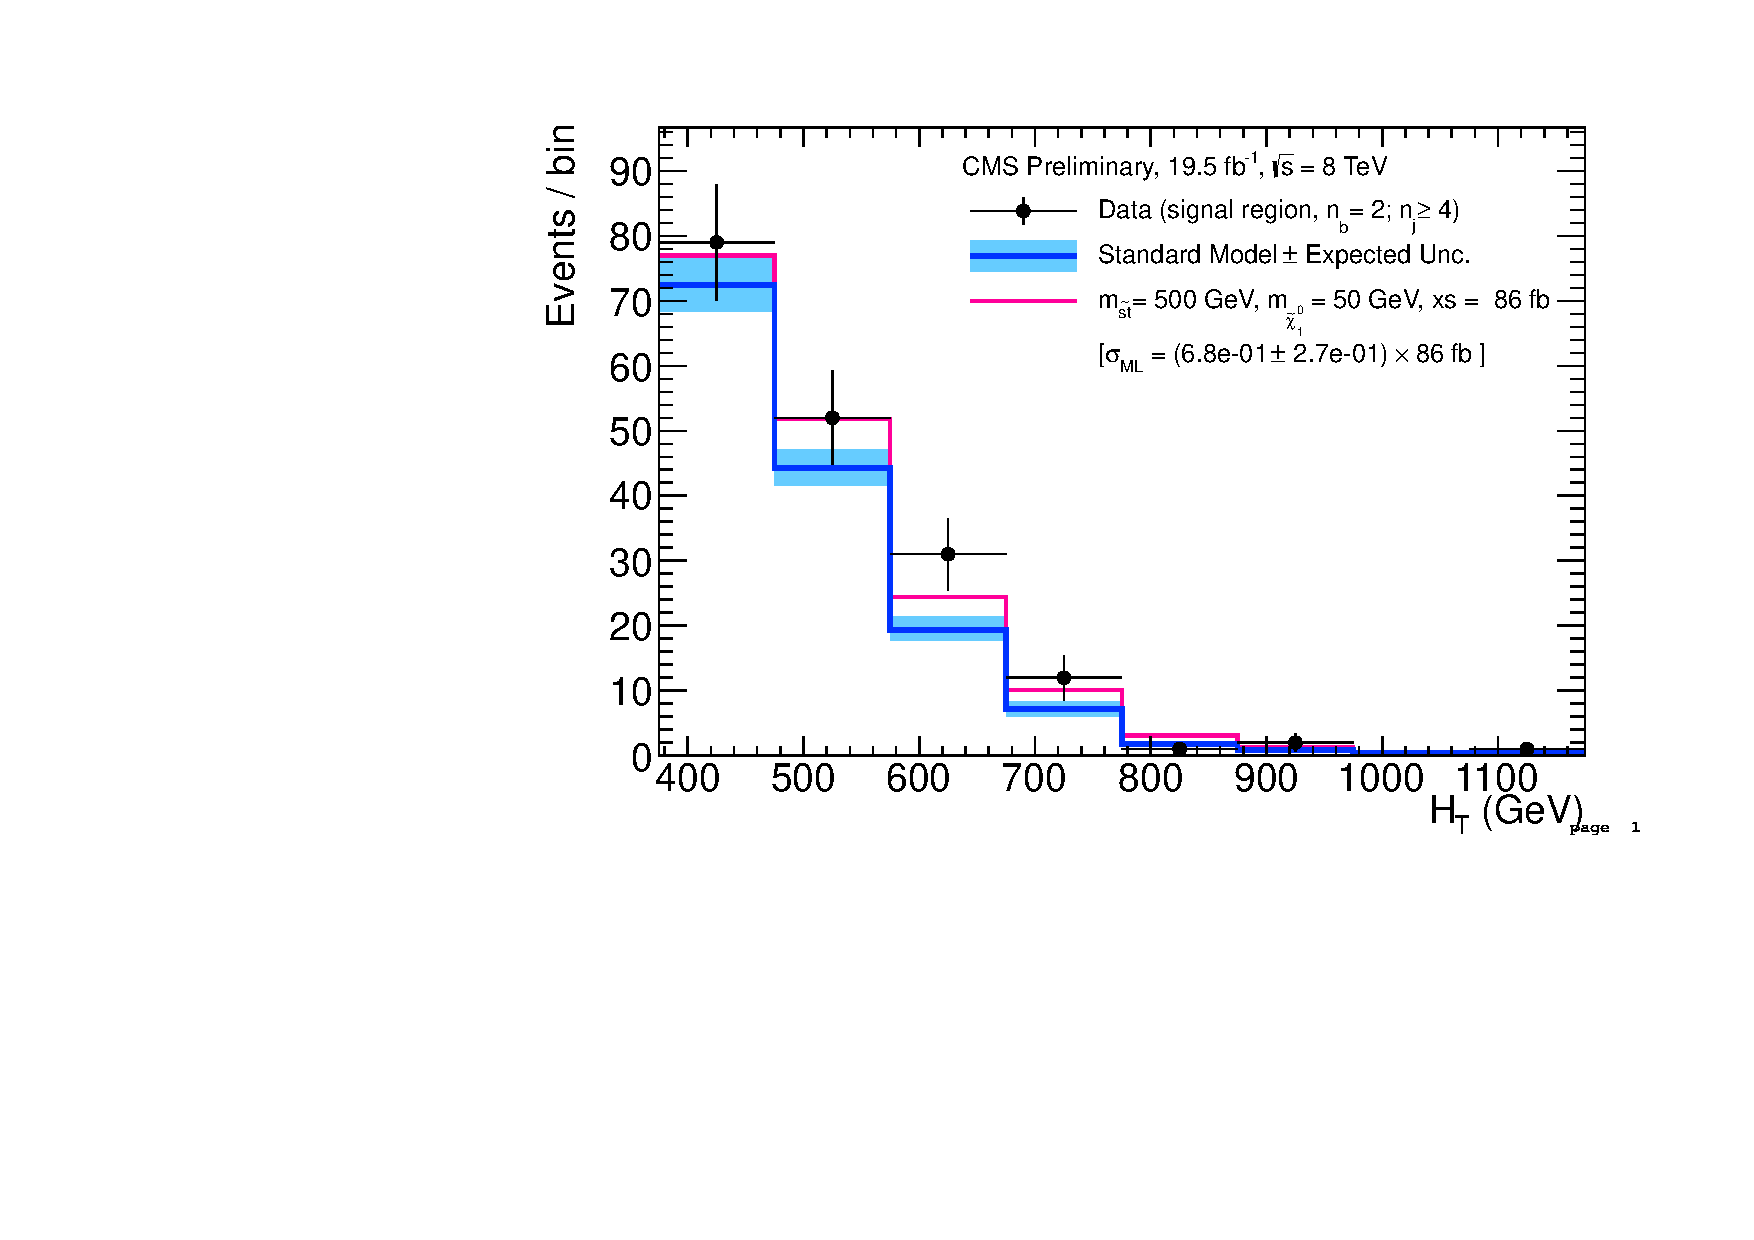
\includegraphics[width=0.45\textwidth]{figures/fit/v22/wSignal/500_50/bestFit_2012pf_RQcdZero_fZinvAll_1b_ge4j-1hp_2b_ge4j-1h_signal_sel2b_ge4j}
    } \\
    \subfigure[\njethigh, $\nb = 1$, simultaneous fit]{
      \includegraphics[width=0.45\textwidth,page=13]{figures/fit/v22/stackedSig/500_50/bestFit_2012pf_RQcdZero_fZinvAll_1b_ge4j-1p_2b_ge4j-1_sel1b_ge4j_smOnly.pdf}
    } 
    \subfigure[\njethigh, $\nb = 2$, simultaneous fit]{
      \includegraphics[width=0.45\textwidth,page=9]{figures/fit/v22/stackedSig/500_50/bestFit_2012pf_RQcdZero_fZinvAll_1b_ge4j-1p_2b_ge4j-1_sel2b_ge4j_smOnly.pdf}
    } \\
    \subfigure[Upper Limit on signal stength, simultaneous fit]{
      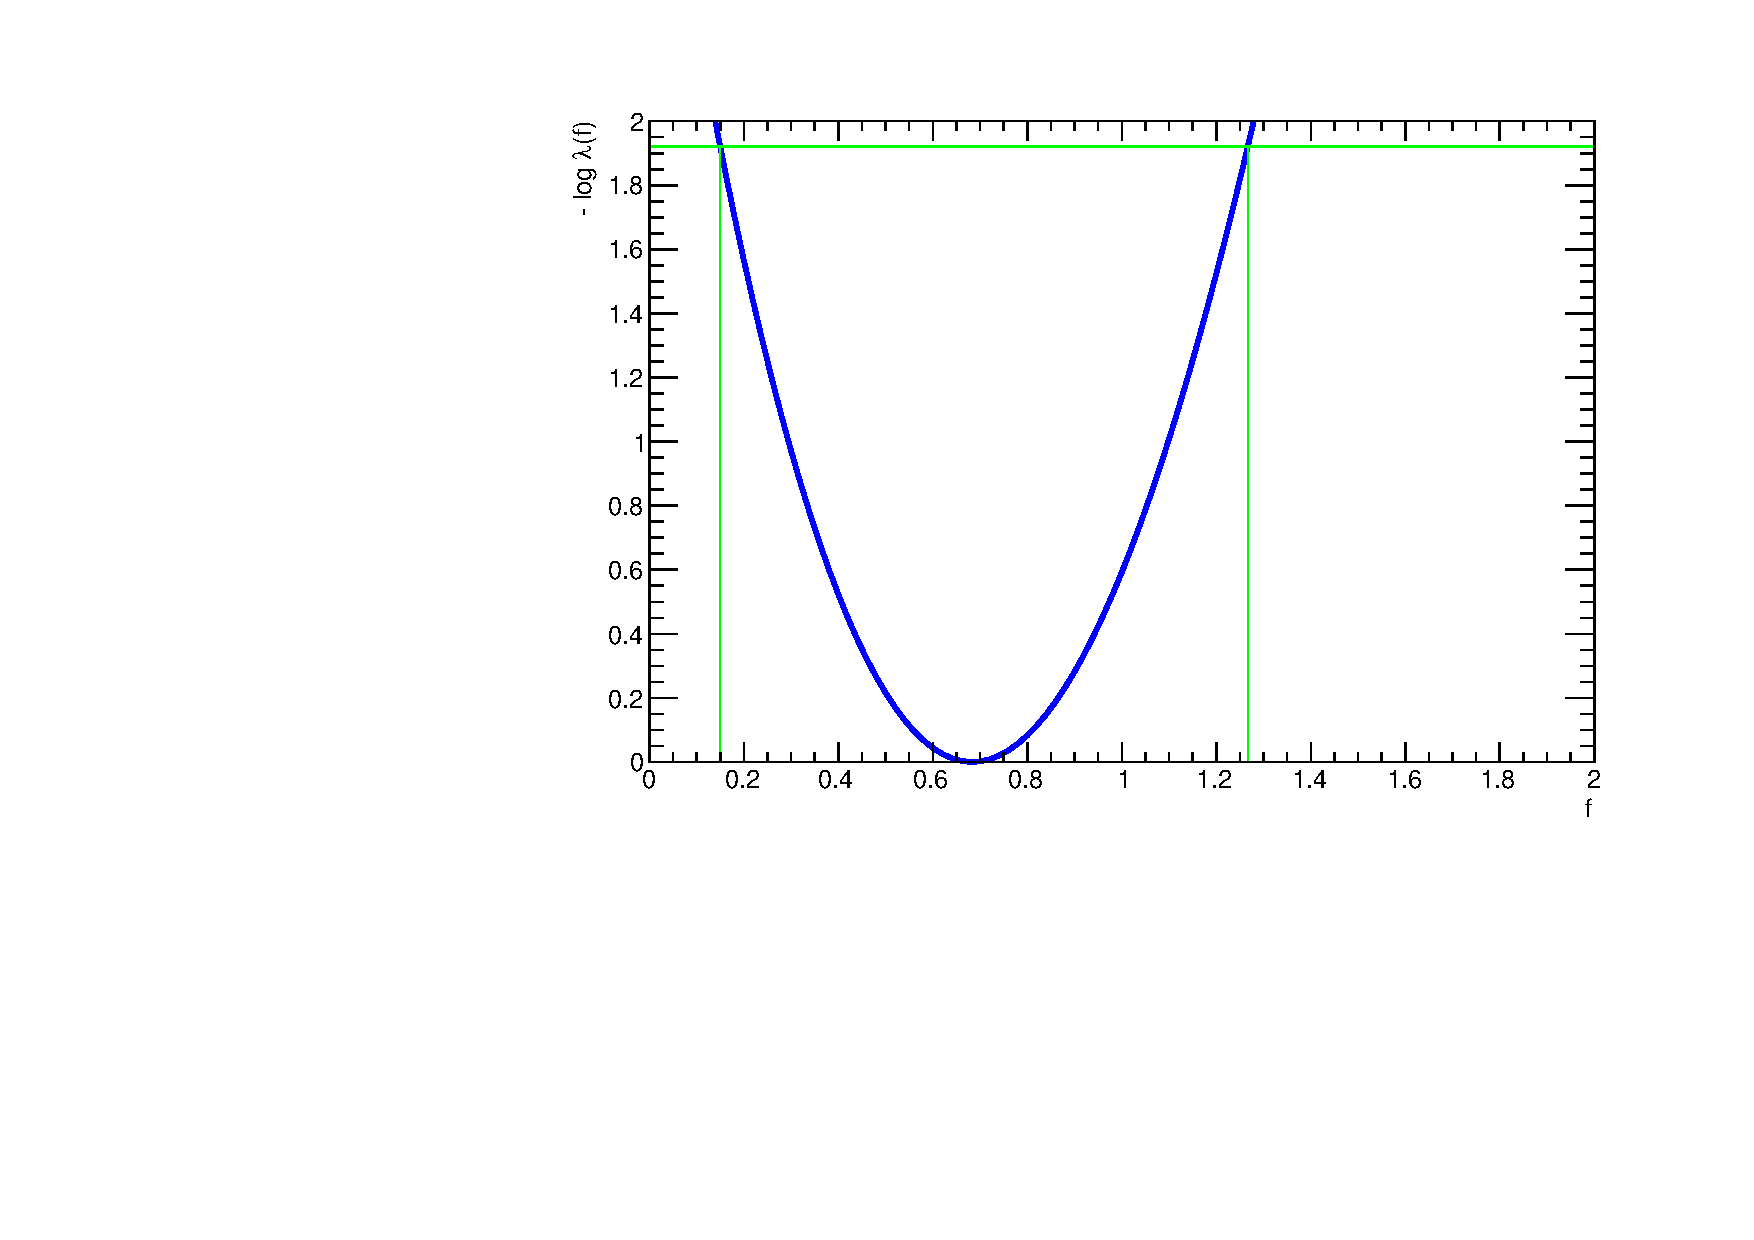
\includegraphics[width=0.45\textwidth]{figures/fit/v22/wSignal/500_50/intervalPlot_2012pf_RQcdZero_fZinvAll_1b_ge4j-1hp_2b_ge4j-1h_signal_95}
    } \\

    \caption{\label{fig:t2cc-best-fit} Comparison of
      the \scalht-binned observed data yields and expectations for the
      hadronic sample, as determined by a simultaneous fit to all data
      samples under the signal plus SM background hypothesis. The
      observed event yields in data (black dots), the SM expectations
      (dark blue solid line), and the signal expectations (pink solid
      line), as determined by the simultaneous fit, are shown. The
      signal model is \texttt{T2cc} with $m_{\sq} = 250\GeV$ and
      $m_{\text{LSP}} = 230\GeV$. Three event categories are
      considered: (Top) \njethigh and $\nb = 0$, (Middle) \njethigh and
      $\nb = 0$, (Bottom) \njethigh and $\nb = 1$. The fit is
      performed (Left) for each individual event category or (Right)
      simultaneously across all three event categories.}
  \end{center}
\end{figure*}

\begin{figure*}[t!]
  \begin{center}
    \subfigure[\njethigh, $\nb = 1$, simultaneous fit]{
      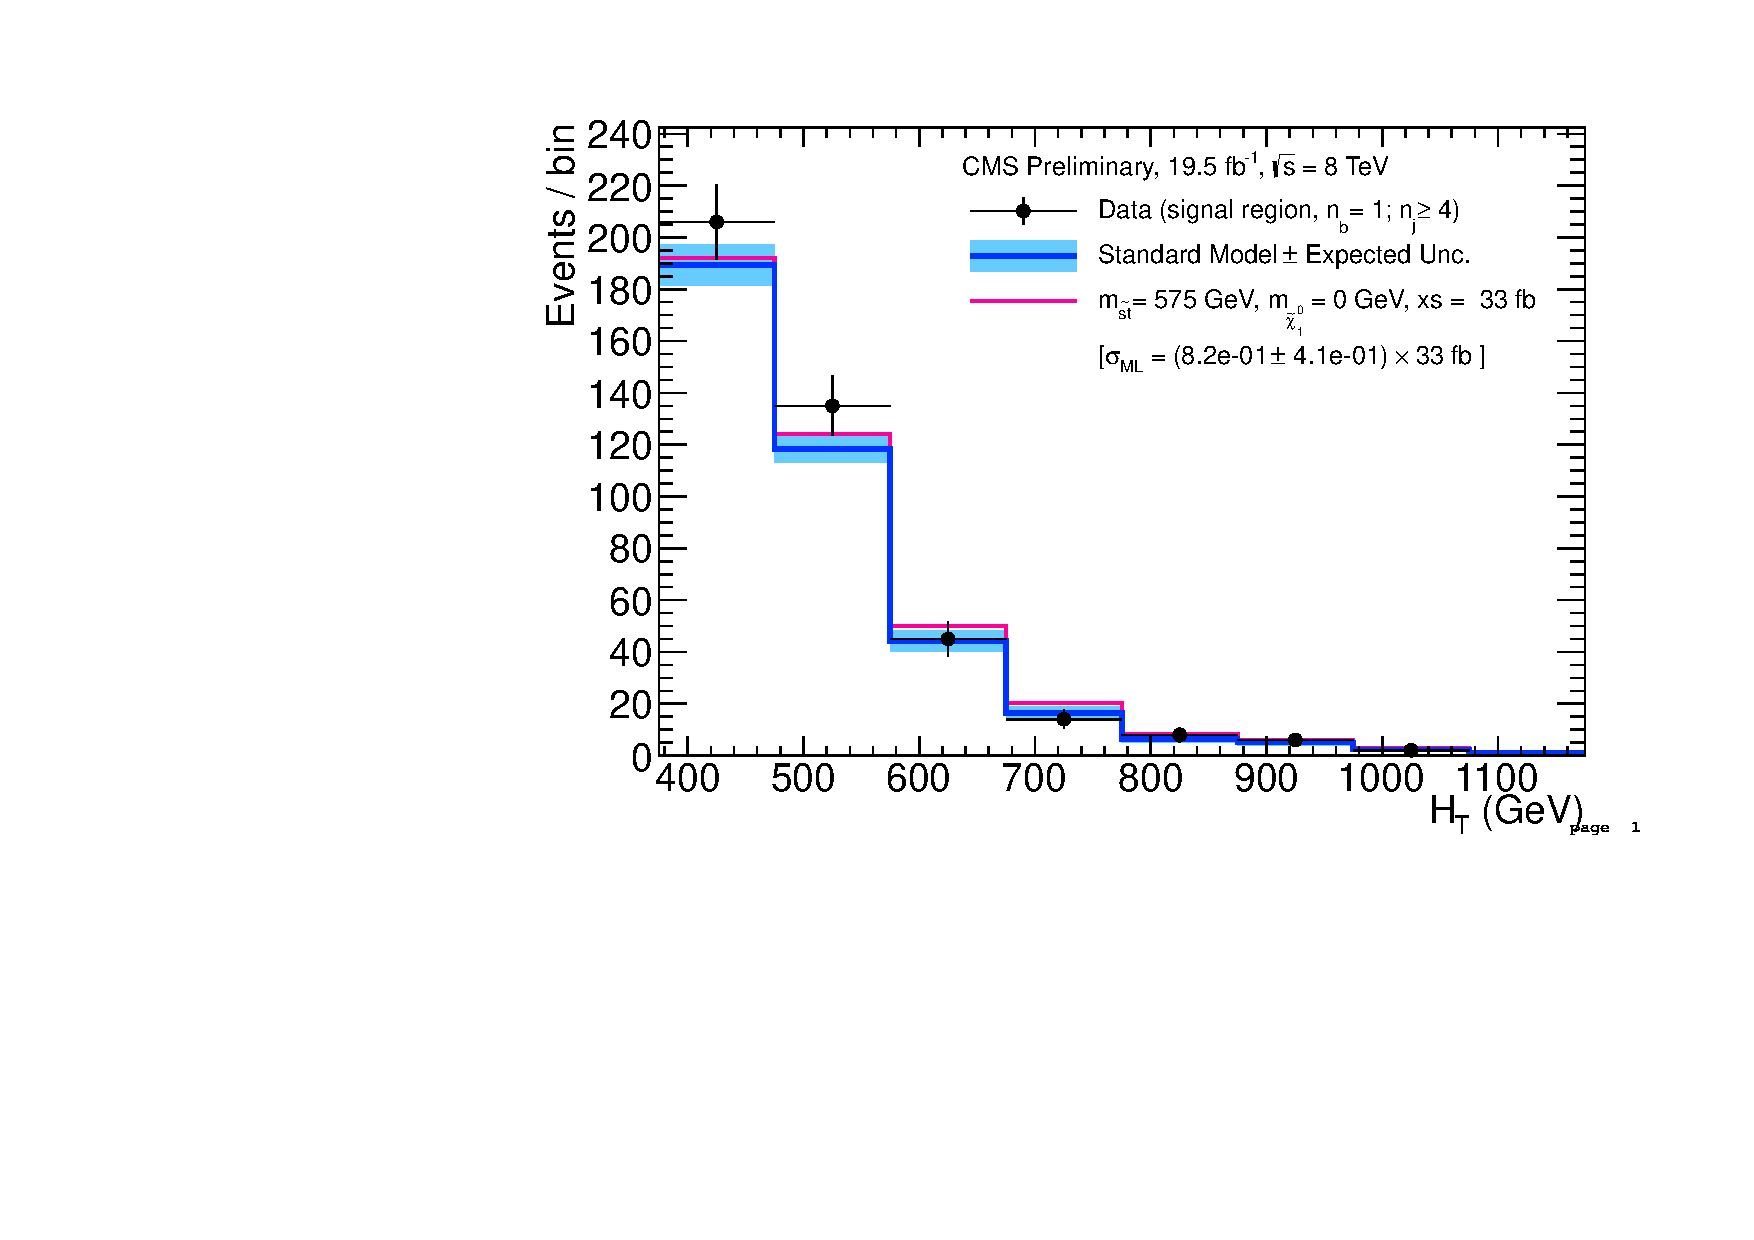
\includegraphics[width=0.45\textwidth]{figures/fit/v22/wSignal/575_0/bestFit_2012pf_RQcdZero_fZinvAll_1b_ge4j-1hp_2b_ge4j-1h_signal_sel1b_ge4j}
    } 
    \subfigure[\njethigh, $\nb = 2$, simultaneous fit]{
      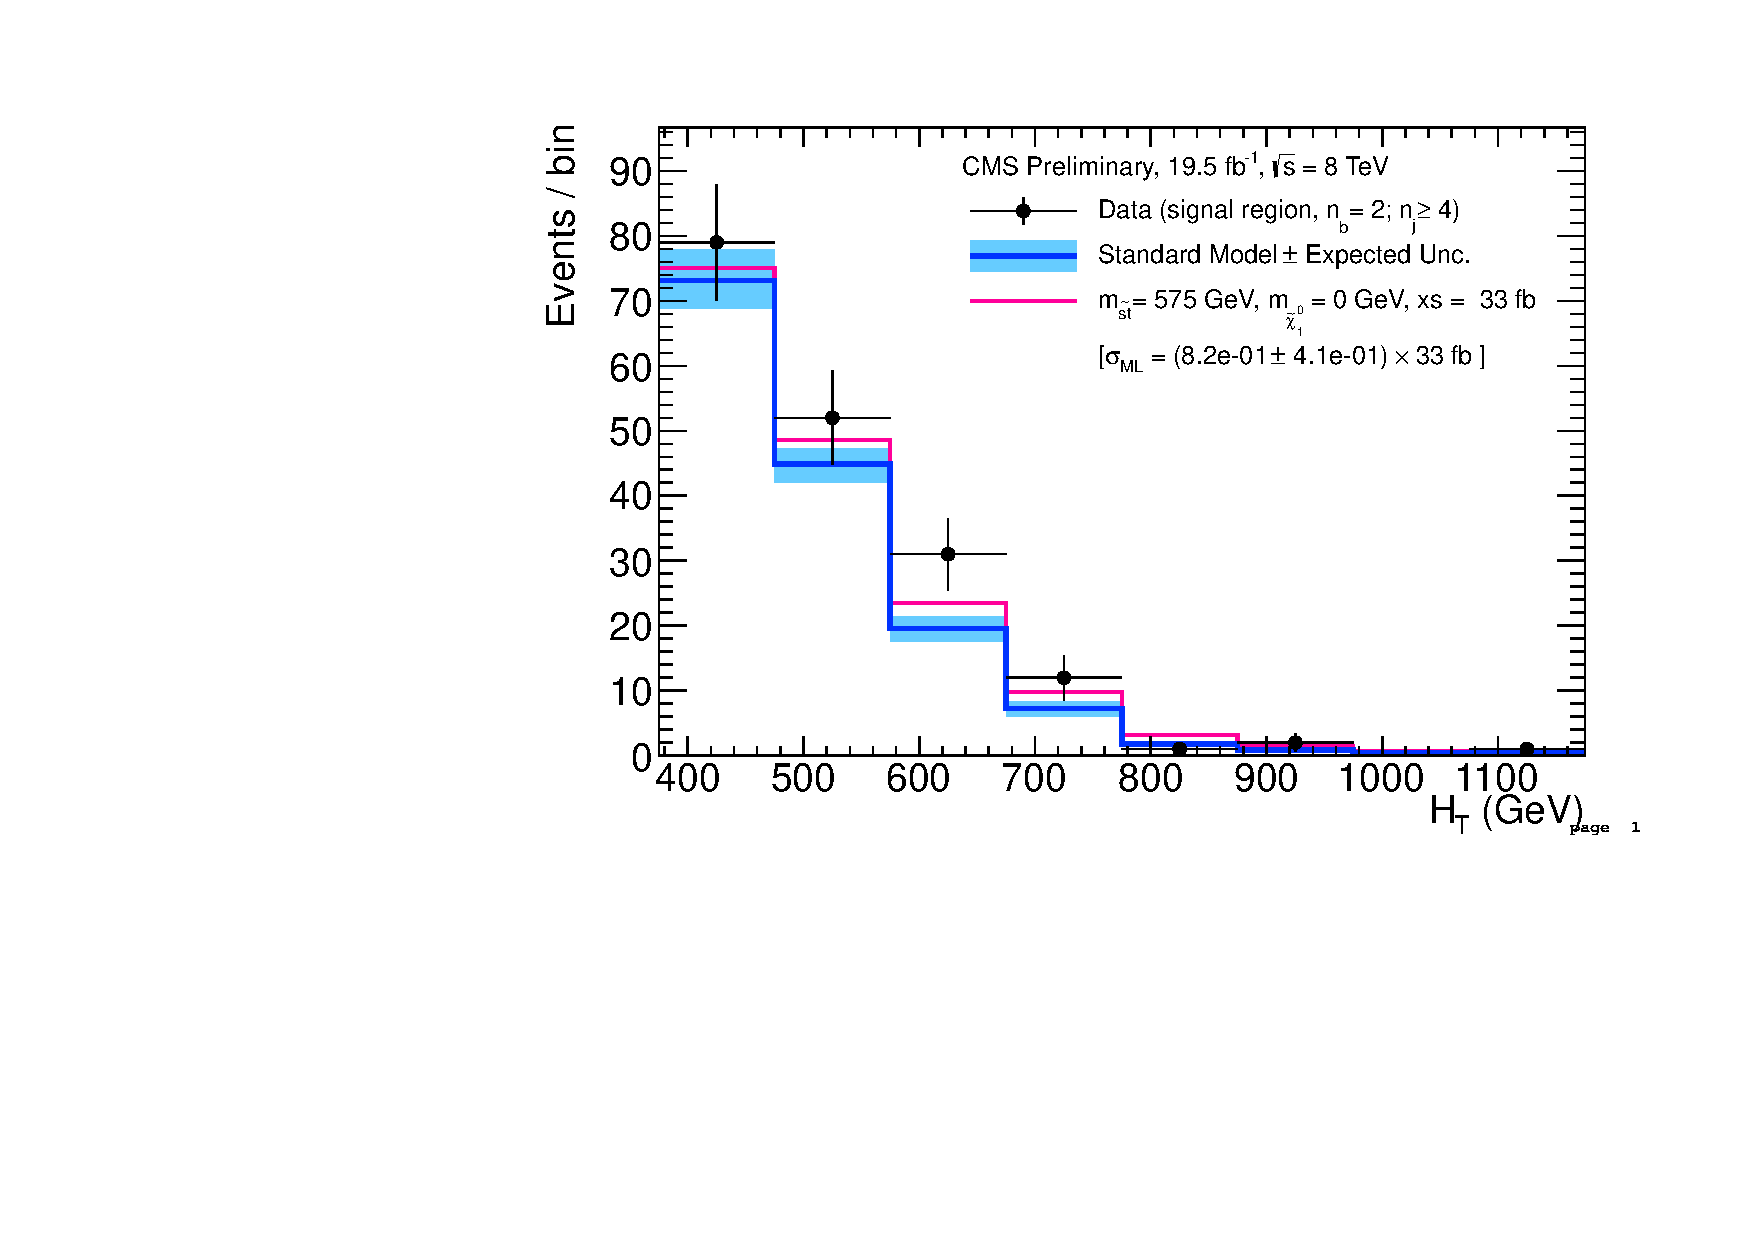
\includegraphics[width=0.45\textwidth]{figures/fit/v22/wSignal/575_0/bestFit_2012pf_RQcdZero_fZinvAll_1b_ge4j-1hp_2b_ge4j-1h_signal_sel2b_ge4j}
    } \\
    \subfigure[\njethigh, $\nb = 1$, simultaneous fit]{
      \includegraphics[width=0.45\textwidth,page=13]{figures/fit/v22/stackedSig/575_0/bestFit_2012pf_RQcdZero_fZinvAll_1b_ge4j-1p_2b_ge4j-1_sel1b_ge4j_smOnly.pdf}
    } 
    \subfigure[\njethigh, $\nb = 2$, simultaneous fit]{
      \includegraphics[width=0.45\textwidth,page=9]{figures/fit/v22/stackedSig/575_0/bestFit_2012pf_RQcdZero_fZinvAll_1b_ge4j-1p_2b_ge4j-1_sel2b_ge4j_smOnly.pdf}
    } \\
    \subfigure[Upper Limit on signal stength, simultaneous fit]{
      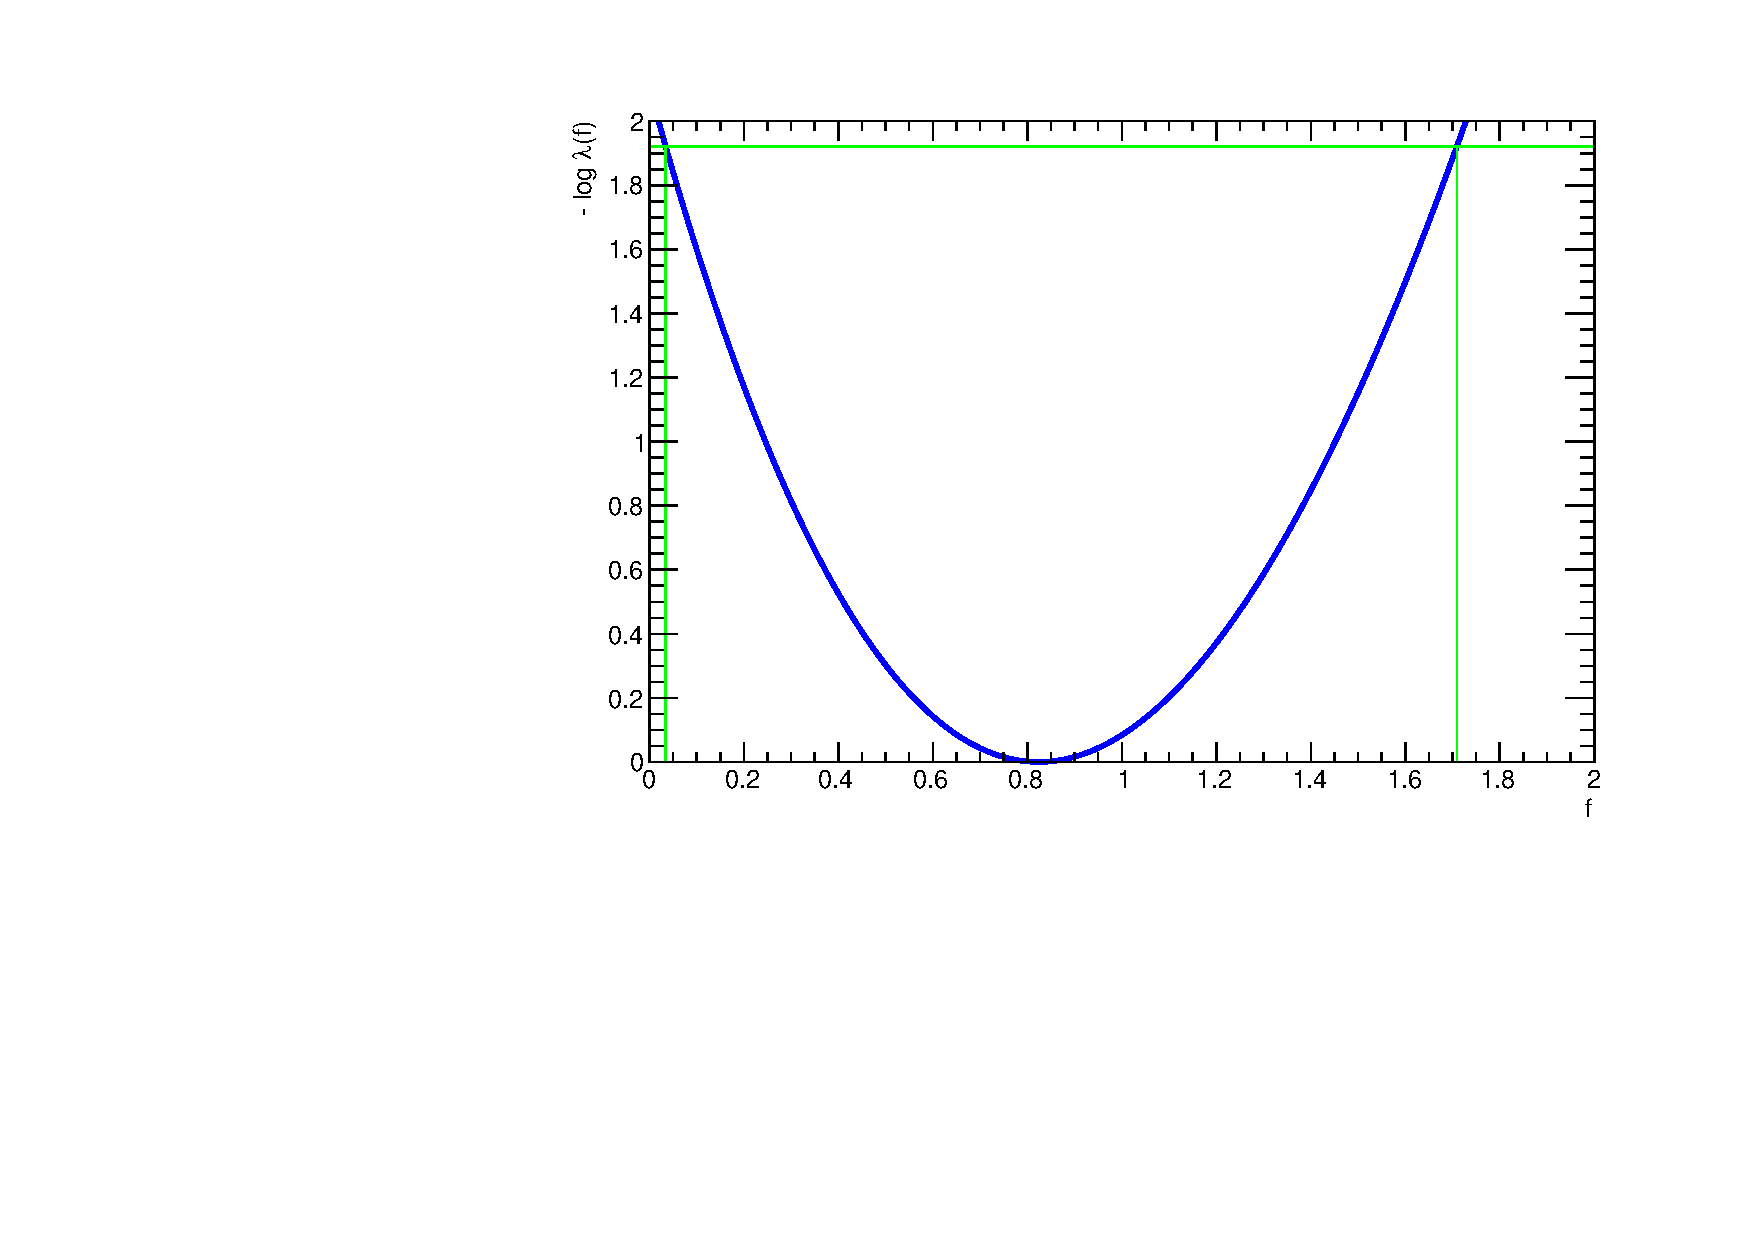
\includegraphics[width=0.45\textwidth]{figures/fit/v22/wSignal/575_0/intervalPlot_2012pf_RQcdZero_fZinvAll_1b_ge4j-1hp_2b_ge4j-1h_signal_95}
    } \\

    \caption{\label{fig:t2cc-best-fit} Comparison of
      the \scalht-binned observed data yields and expectations for the
      hadronic sample, as determined by a simultaneous fit to all data
      samples under the signal plus SM background hypothesis. The
      observed event yields in data (black dots), the SM expectations
      (dark blue solid line), and the signal expectations (pink solid
      line), as determined by the simultaneous fit, are shown. The
      signal model is \texttt{T2cc} with $m_{\sq} = 250\GeV$ and
      $m_{\text{LSP}} = 230\GeV$. Three event categories are
      considered: (Top) \njethigh and $\nb = 0$, (Middle) \njethigh and
      $\nb = 0$, (Bottom) \njethigh and $\nb = 1$. The fit is
      performed (Left) for each individual event category or (Right)
      simultaneously across all three event categories.}
  \end{center}
\end{figure*}


%%Figure~\ref{fig:limits-sms} shows the upper limit on the cross section
%%at 95\% CL as a function of $m_{\sq}$ or $m_{\gl}$ and $m_{\rm LSP}$
%%for various simplified models. The point-to-point fluctuations are due
%%to the finite number of pseudo-experiments used to determine the
%%observed upper limit. The solid thick black line indicates the
%%observed exclusion region assuming NLO+NLL~\cite{Beenakker:1996ch,
%%  susy-nlo-nll} SUSY cross section for squark pair production in the
%%limit of very massive gluinos (or vice versa). The thin black lines
%%represent the observed excluded region when varying the cross section
%%by its theoretical uncertainty. The dashed purple lines indicate the
%%median (thick line) $\pm 1 \sigma$ (thin lines) expected exclusion
%%regions.
%
%%The estimates on mass limits are determined conservatively from the
%%observed exclusion based on the theoretical production cross section
%%minus $1\sigma$ uncertainty.  The most stringent mass limits on
%%pair-produced sparticles are obtained at low LSP masses, while the
%%limits typically weaken for compressed spectra, \ie, points close to
%%the diagonal. In particular, for all of the considered simplified
%%models, there is an LSP mass beyond which no limit can be set. This is
%%illustrated in Figure~\ref{fig:t1}, where the most stringent limit on
%%the gluino mass of $950\GeV$ is obtained for low LSP masses. This
%%limit only weakens to $900\GeV$ when the LSP mass reaches
%%$425\GeV$. However, for LSP masses above $450\GeV$, no mass range can
%%be excluded for gluinos decaying to first- or second-generation
%%quarks. Table~\ref{tab:sms} summarises the mass limits obtained from
%%the considered simplified models.
%%
%%\begin{figure}[h!]
%%  \begin{center}
%%    \subfigure[\label{fig:t1}$\sGlu\sGlu\,\rightarrow\,\textrm{q}\bar{\textrm{q}}\chiz \textrm{q}\bar{\textrm{q}}\chiz$ (Model \texttt{T1})]{
%%      \includegraphics[width=0.45\textwidth]{figures/limits/v4/t1}
%%    } \quad
%%    \subfigure[\label{fig:t2}$\sQua\sQua\,\rightarrow\,\textrm{q}\chiz \bar{\textrm{q}}\chiz$ (Model \texttt{T2})]{ 
%%      \includegraphics[width=0.45\textwidth]{figures/limits/v4/t2}
%%    } \\
%%%    \subfigure[\label{fig:t2tt}$\sTop\sTop\,\rightarrow\,\textrm{t}\chiz \bar{\textrm{t}}\chiz$ (Model \texttt{T2tt})]{ 
%%%      \includegraphics[width=0.45\textwidth]{figures/limits/v1/t2tt}
%%%    } \quad 
%%    \subfigure[\label{fig:t2bb}$\sBot\sBot\,\rightarrow\,\textrm{b}\chiz \bar{\textrm{b}}\chiz$ (Model \texttt{T2bb})]{ 
%%      \includegraphics[width=0.45\textwidth]{figures/limits/v4/t2bb}
%%    } \\
%%    \subfigure[\label{fig:t1tttt}$\sGlu\sGlu\,\rightarrow\,\textrm{t}\bar{\textrm{t}}\chiz \textrm{t}\bar{\textrm{t}}\chiz$ (Model \texttt{T1tttt})]{
%%      \includegraphics[width=0.45\textwidth]{figures/limits/v4/t1tttt}
%%    } \quad 
%%    \subfigure[\label{fig:t1bbbb}$\sGlu\sGlu\,\rightarrow\,\textrm{b}\bar{\textrm{b}}\chiz \textrm{b}\bar{\textrm{b}}\chiz$ (Model \texttt{T1bbbb})]{
%%      \includegraphics[width=0.45\textwidth]{figures/limits/v4/t1bbbb}
%%    } \\
%%    \caption{\label{fig:limits-sms} Upper limit on cross section at
%%      95\% CL as a function of $m_{\sq}$ or $m_{\gl}$ and $m_{\rm
%%        LSP}$ for various simplified models. The solid thick black
%%      line indicates the observed exclusion region assuming NLO+NLL
%%      SUSY production cross section. The thin black lines represent
%%      the observed excluded region when varying the cross section by
%%      its theoretical uncertainty. The dashed purple lines indicate
%%      the median (thick line) $\pm 1 \sigma$ (thin lines) expected
%%      exclusion regions. 
%%      %The mass ranges considered for models \texttt{T2tt} and
%%      %\texttt{T1tttt} differ from the other models.  
%%    }
%%  \end{center}
%%\end{figure}
%%
%%\begin{figure*}[t!]
%%  \begin{center}
%%    \includegraphics[width=0.45\textwidth]{figures/limits/v4/T2tt_mlsp0_xmin300_smooth5_prelim.pdf} \,
%%    \includegraphics[width=0.45\textwidth]{figures/limits/v4/T2tt_mlsp50_xmin300_smooth5_prelim.pdf}  \\
%%    \includegraphics[width=0.45\textwidth]{figures/limits/v4/T2tt_mlsp100_xmin300_smooth5_prelim.pdf} \,
%%    \includegraphics[width=0.45\textwidth]{figures/limits/v4/T2tt_mlsp150_xmin350_smooth5_prelim.pdf} \\
%%    \caption{\label{fig:t2tt-1d} Excluded cross sections versus top
%%      squark mass $m_{\sTop}$ for the model \texttt{T2tt}, in which
%%      pair-produced top squarks each decay to a top quark and the LSP
%%      with a mass $m_{\rm LSP} = 0\gev$ (top left), $m_{\rm LSP} =
%%      50\gev$ (top right), $m_{\rm LSP} = 100\gev$ (bottom left),
%%      $m_{\rm LSP} = 150\gev$ (bottom right). The observed upper limit
%%      (95\% CL) on the production cross section is shown as a function
%%      of $m_{\sTop}$ (solid line), along with the expected upper limit
%%      and $\pm1\sigma$ experimental uncertainties (long-dashed line
%%      with shaded band), and the NLO+NLL top squark pair-production
%%      cross section and theoretical uncertainties (dotted line with
%%      shaded band).}
%%  \end{center}
%%\end{figure*}
%%
%%Figure~\ref{fig:t2tt-1d} shows the observed upper limit at 95\% CL on
%%the production cross section as a function of the top squark mass
%%($m_{\sTop}$) for the model \texttt{T2tt} when considering different
%%LSP masses in the range 0--150\GeV. No exclusion on possible top
%%squark masses is observed when considering the theoretical production
%%cross section minus $1\sigma$ uncertainty. However, the expected
%%exclusion covers the ranges 300--520\GeV, 320--520\GeV, and
%%420-480\GeV for $m_{\text{LSP}} = 0\GeV$, $m_{\text{LSP}} = 50\GeV$,
%%and $m_{\text{LSP}} = 100\GeV$ respectively. No exclusion is expected
%%for the LSP with a mass greater than 100\GeV.
%%%The expected reach for the T2tt model is summarised
%%%in Table~\ref{tab:sms-reach}. 
